\documentclass[11pt]{article}
\usepackage[a4paper,margin=2.2cm]{geometry}
\usepackage{amsmath,amssymb}
\usepackage{graphicx}
\usepackage{booktabs}
\usepackage{tabularx}
\usepackage{xcolor}
\usepackage[colorlinks=true,linkcolor=blue!50!black,urlcolor=blue!50!black,citecolor=blue!50!black]{hyperref}
\usepackage{caption}
\captionsetup{font=small,labelfont=bf}
\setlength{\emergencystretch}{2em}
\newcolumntype{L}{>{\raggedright\arraybackslash}X}
\usepackage{url}
\def\UrlBreaks{\do\/\do\_\do\.\do-}
\DeclareUrlCommand\file{\urlstyle{tt}}
\newcommand{\Dr}{\Delta\rho}

\title{Coherent phonons in EDUS:\\ Ehrenfest dynamics of the lattice at $\Gamma$ with the coupling of EPW}
\author{EDUS development notes, branch \texttt{ehrenfest}}
\date{\today}

\begin{document}
\maketitle

\begin{abstract}
EDUS now propagates the displacements of the atoms at $q=\Gamma$ together with the density matrix of the electrons,
at the mean-field (Ehrenfest) level. The electrons feel the displaced lattice through the electron--phonon coupling
$g_\mu=\partial H/\partial u_\mu$, read in the Wannier representation from the files of EPW; the atoms feel the force
of the excited electrons, with masses and force constants from the dynamical matrix of ph.x. These notes describe the
equations that are solved, every file that was added or changed and what it contains, the input and output, and the
validation on a synthetic hBN model and on the real hBN from QE and EPW: the frequency of the free lattice, the softening by the electrons and its static
limit, the conservation of energy, the coherent phonon driven by a laser, the independence of the number of MPI ranks
and the convergence in the time step. The last section lists what is not implemented yet.
\end{abstract}

\tableofcontents

\section{What is solved}
The full theory (Hamiltonian, mean-field argument, bare vs screened quantities, general $q$) is in
\file{src/Phonons/EHRENFEST.md}. Only the equations actually implemented are summarized here.

\paragraph{Only $\Gamma$.} In the mean field the force on the mode $q$ comes from the coherences between $k$ and $k-q$.
EDUS propagates $\rho(k)$ diagonal in $k$, which is exact as long as the system stays translationally invariant: a laser
in the dipole approximation and a displacement at $q=0$ preserve it, so only the $\Gamma$ phonons are driven. The data
structures are indexed by $q$, but the input accepts only $q=\Gamma$.

\paragraph{Coordinates.} Instead of the normal modes, the code uses the cartesian displacements of the atoms,
$u_\mu$ with $\mu = 3\kappa+\alpha$ (atom $\kappa$, direction $\alpha$), in bohr. This is the basis in which EPW writes
the coupling, so no rotation to the modes and no zero-point lengths $\ell_\nu$ are needed.

\paragraph{Equations of motion.} With $\Dr=\rho-\rho_0$,
\begin{align}
i\dot\rho(k) &= \Big[H_e(k,t) + \sum_\mu u_\mu\, g_\mu(k),\ \rho(k)\Big] + \text{(gradient term, as before)},\\
M_\mu \ddot u_\mu &= -\sum_\nu K_{\mu\nu}\,u_\nu \;-\; F_\mu \;-\; \frac{2M_\mu}{\tau}\,\dot u_\mu ,\\
F_\mu &= \frac{s}{N}\sum_k \mathrm{Tr}\big[g_\mu(k)\,\Dr(k)\big] \;=\; s\sum_R\sum_{mn} g_{\mu,mn}(R)\,\Dr_{mn}(R)^* ,
\label{eq:force}
\end{align}
where $H_e = H_0+\mathbf E\cdot\mathbf r+\Sigma[\Dr]$ is the Hamiltonian EDUS already propagated, $g_\mu$ is in Ha/bohr,
$K$ in Ha/bohr$^2$, $M_\mu$ is the mass of the atom of $\mu$, $s$ the spin degeneracy, $N$ the number of $k$ points and
$\tau$ an optional phenomenological damping time. Only $\Dr$ exerts a force: at equilibrium the geometry is relaxed. The
second form of~\eqref{eq:force} (Parseval with the EDUS convention $O(k)=\sum_R e^{ik\cdot R}O(R)$) is the one used:
each rank sums its local $R$ points and the result is reduced.

\paragraph{Energy.} Per unit cell, $E = s\big(\mathrm{Tr}[H_0\Dr]+\tfrac12\mathrm{Tr}[\Sigma\Dr]\big)/N + u\cdot F +
\tfrac12\sum_\mu M_\mu\dot u_\mu^2+\tfrac12 u\cdot K u$ changes only because of the work of the field. This was checked
by differentiating it with the equations above, and numerically (section~\ref{sec:validation}).

\paragraph{Force constants: bare or Born--Oppenheimer.} ph.x gives the Born--Oppenheimer force constants $K^{\rm BO}$,
which already contain the screening by the electrons. Since the electrons are propagated explicitly, they generate this
screening again, and using $K^{\rm BO}$ with the whole $\Dr$ counts it twice. How this is treated is the subject of
section~\ref{sec:adiabatic}.

\section{\texorpdfstring{Screening of $g$ and $K$ at a glance}{Screening of g and K at a glance}}\label{sec:screening}
The perturbation of a displaced atom is screened in three layers: the bare ionic potential $\partial V_{\rm ion}$, the
response of the bands \emph{outside} the Wannier model (core-like and high-energy bands), and the response of the
electrons \emph{of} the model. DFPT (ph.x, EPW) contains all three, statically. EDUS generates the third one again,
dynamically, through $\Sigma[\Dr]$ (Hartree + SEX); the first two it cannot generate. So the quantities to give to EDUS
are those screened by everything \emph{except} the electrons of the model (as in constrained RPA/DFPT), for the
coupling and for the force constants alike (table~\ref{tab:layers}).

Notation: $\chi_0$ is the independent-particle static response of the model, $\delta\rho_{nm}=
\frac{f_n-f_m}{\varepsilon_n-\varepsilon_m}V_{nm}$ (Bloch gauge); $\Sigma$ the (linear) mean-field kernel;
$\chi=(1-\chi_0\Sigma)^{-1}\chi_0$ the interacting response of the model; $\langle A\,B\rangle_{\mu\nu} =
\frac sN\sum_k\mathrm{Tr}[A_\mu B_\nu]$.

\begin{table}[h]
\centering\small
\begin{tabularx}{\textwidth}{l c c c L}
\toprule
Quantity & $\partial V_{\rm ion}$ & outside & model & Where it comes from / role in EDUS \\
\midrule
$g^{\rm ion}$ (fully bare) & \checkmark & -- & -- & EPW with \texttt{lnoloc} (refused by ph.x). \textbf{Never right}: loses the outside screening. \\
$g^{\rm b}$ (bare w.r.t.\ the model) & \checkmark & \checkmark & -- & $g^{\rm s}-\Sigma[\chi_0g^{\rm s}]$. \textbf{Goes in $H$} with the mean field. \\
$g^{\rm s}$ (screened) & \checkmark & \checkmark & \checkmark\,(DFT) & EPW (\texttt{dvscf}). Goes in $H$ in IPA. \\
\midrule
$K^0$ (clamped model electrons) & \checkmark & \checkmark & -- & $K^{\rm BO}-\Pi$. \textbf{Used with the whole $\Dr$} (\texttt{static}). \\
$K^{\rm BO}$ (Born--Oppenheimer) & \checkmark & \checkmark & \checkmark\,(DFT) & ph.x. Used with $\rho-\rho_{\rm BO}$ (\texttt{dynamic}). \\
\bottomrule
\end{tabularx}
\caption{Which layers of screening each quantity contains. The rows in bold are the ones consistent with electrons
that are propagated with their own mean field: the third layer is supplied by EDUS, not by the input.}
\label{tab:layers}
\end{table}

\paragraph{The same operation on $g$ and on $K$.} In the static limit the displacement $u_\nu$ makes the electrons of
the model respond with $\delta\rho_\nu$. This response does two things: it adds the induced potential $\Sigma[\delta\rho_\nu]$
to what the electrons feel (screening of $g$), and it exerts the force $\langle g\,\delta\rho_\nu\rangle$ on the atoms
(softening of $K$). Removing the screening means removing both, and with the unscreened coupling the response is simply
\begin{equation}
\delta\rho_\nu = \chi\,g^{\rm b}_\nu = \chi_0\big(g^{\rm b}_\nu+\Sigma[\delta\rho_\nu]\big) = \chi_0\,g^{\rm s}_\nu ,
\end{equation}
since $g^{\rm b}+\Sigma[\delta\rho]=g^{\rm s}$ by construction (this is the check printed in the recap). Table~\ref{tab:remove}
compares the two operations.

\begin{table}[h]
\centering\small
\begin{tabularx}{\textwidth}{l L L}
\toprule
 & Coupling $g$ (what the electrons feel) & Force constants $K$ (what the atoms feel) \\
\midrule
From DFPT & $g^{\rm s}$ (EPW) & $K^{\rm BO}$ (ph.x) \\
Added again by the model & $\Sigma[\delta\rho]$: $\;g^{\rm b}\to g^{\rm b}+\Sigma[\delta\rho]$ & $\Pi$: $\;K^0\to K^0+\Pi$ \\
To remove & $\Sigma[\chi_0 g^{\rm s}]$ & $\Pi = \langle g^{\rm b}\,\chi\,g^{\rm b}\rangle = \langle g^{\rm b}\,\chi_0\,g^{\rm s}\rangle\;\le 0$ \\
Result & $g^{\rm b} = g^{\rm s}-\Sigma[\chi_0 g^{\rm s}]$ & $K^0 = K^{\rm BO}-\Pi$ \\
How & closed formula, one $\chi_0$ and one $\Sigma$ per mode & self-consistent $\delta\rho$ (linear mixing), then the trace \\
Option & \texttt{coupling = "screened"} (default) & \texttt{adiabatic\_reference = "static"}; or \texttt{"dynamic"}: keep $K^{\rm BO}$ and subtract $\rho_{\rm BO}(t)$ in the force \\
Function & \texttt{Lattice::unscreen\_coupling} & \texttt{Lattice::static\_response} \\
In IPA ($\Sigma=0$) & nothing to do: $g^{\rm b}=g^{\rm s}$ & still needed: $\Pi^{\rm IPA}=\langle g^{\rm s}\chi_0 g^{\rm s}\rangle$ \\
Synthetic hBN, HSEX & correction of 35\% on $g$ & without it 1370 $\to$ 1006 cm$^{-1}$ \\
\bottomrule
\end{tabularx}
\caption{Removing the screening of the electrons of the model from the coupling and from the force constants. The
order matters: $g$ is unscreened first, and $\Pi$ is then computed with $g^{\rm b}$.}
\label{tab:remove}
\end{table}

\paragraph{Why $K$ must be corrected even in IPA, and $g$ not.} The electrons of EDUS always respond to $u$, also
without the mean field, so they always add $\Pi$ to the lattice. Without the mean field, instead, their response does
not change the potential they feel, so they add nothing to $g$: $g^{\rm s}$ is already what they should feel.

\paragraph{Combinations.} Static limit (no laser) of each choice with the mean field on; ``electrons feel'' is the total
perturbation $g+\Sigma[\delta\rho]$, ``lattice'' the effective force constants (table~\ref{tab:combos}).

\begin{table}[h]
\centering\small
\begin{tabularx}{\textwidth}{l l L L}
\toprule
\texttt{coupling} & \texttt{adiabatic\_reference} & Electrons feel & Lattice \\
\midrule
\texttt{screened} & \texttt{static} / \texttt{dynamic} & $g^{\rm s}$ \hfill\checkmark & $K^{\rm BO}$ \hfill\checkmark \\
\texttt{screened} & \texttt{none} & $g^{\rm s}$ \hfill\checkmark & $K^{\rm BO}+\Pi$: softened twice \\
\texttt{bare} (files are $g^{\rm s}$) & \texttt{static} / \texttt{dynamic} & $g^{\rm s}+\Sigma[\chi g^{\rm s}]$: screened twice & $K^{\rm BO}$ (by construction) \\
\texttt{bare} (files are $g^{\rm s}$) & \texttt{none} & screened twice & softened twice \\
\texttt{bare} (files are $g^{\rm b}$, synthetic) & \texttt{static} / \texttt{dynamic} & $g^{\rm b}+\Sigma[\chi g^{\rm b}]$ \hfill\checkmark & $K^{\rm BO}$ \hfill\checkmark \\
\bottomrule
\end{tabularx}
\caption{Static limit of the options with the mean field. In IPA the two values of \texttt{coupling} coincide and only
the reference matters. \texttt{static} and \texttt{dynamic} differ only in the non-adiabatic response during the
propagation (section~\ref{sec:adiabatic}).}
\label{tab:combos}
\end{table}

\paragraph{What is approximated.} The outside layer is kept static and at the DFT level (it is at high energy); the
response of the model is that of its mean field (the $W$ of the model), not the Hxc of DFT. This does not change the
static limit, which is DFPT by construction for both $g$ and $K$, but it changes $g^{\rm b}$ and $K^0$ themselves, and
therefore the dynamics away from the static limit.

\section{Only the excited electrons push the atoms: the adiabatic reference}\label{sec:adiabatic}
\paragraph{Derivation.} With the bare coupling and the bare force constants $K^0$ the equation of motion is
$M\ddot u = -K^0u - \frac sN\sum_k\mathrm{Tr}[g\,\Dr]$. Split the response of the electrons into the adiabatic
(Born--Oppenheimer) part, which follows the lattice, and the rest:
\begin{equation}
\Dr = \Dr_{\rm BO}(u) + \Dr_{\rm exc},\qquad \frac sN\sum_k\mathrm{Tr}[g_\mu\,\Dr_{\rm BO}] = \sum_\nu\Pi_{\mu\nu}u_\nu ,
\end{equation}
where $\Pi$ is the static response of the electrons, so that $K^{\rm BO} = K^0 + \Pi$. The equation becomes exactly
\begin{equation}
M_\mu\ddot u_\mu = -\sum_\nu K^{\rm BO}_{\mu\nu}u_\nu - \frac sN\sum_k\mathrm{Tr}\big[g_\mu\,(\rho-\rho_0-\Dr_{\rm BO})\big]:
\end{equation}
the force constants are those of ph.x, and only the excited part of the density matrix,
total $-$ ground state $-$ Born--Oppenheimer, pushes the atoms. The advantage is that $\Pi$ never has to be known:
the electrons of the model provide it, with the same Hamiltonian ($H_0$, Hartree, SEX), so it is the interacting response
of the model, and the static limit reproduces the phonons of DFPT by construction. The option
\texttt{adiabatic\_reference} chooses $\Dr_{\rm BO}$.

\paragraph{\texttt{"none"}.} $\Dr_{\rm BO}=0$ with $K^{\rm BO}$: the response is counted twice, and the
lattice is softened (with HSEX from 1370 to 1006 cm$^{-1}$ in the test model).

\paragraph{\texttt{"static"} (default).} $\Dr_{\rm BO} = \sum_\mu u_\mu\,\delta\rho_\mu$, with $\delta\rho_\mu$ the static linear
response of the electrons of the model per unit displacement, computed at the beginning as the self-consistent solution
of (Bloch gauge)
\begin{equation}
\delta\rho_{\mu,nm}(k) = \frac{f_n-f_m}{\varepsilon_n-\varepsilon_m}\,\big(g_\mu + \Sigma[\delta\rho_\mu]\big)_{nm}(k),
\end{equation}
where $\Sigma$ is the same self energy of the propagation (linear in $\delta\rho$), and a single step without the mean
field. It is solved with linear mixing (halved when the change grows), to a relative change of $10^{-10}$ (23 iterations
for hBN with HSEX). Since $\Dr_{\rm BO}$ is linear in $u$, subtracting it in the force is identical to using
$K^0 = K^{\rm BO}-\Pi$, $\Pi_{\mu\nu}=\frac sN\sum_k\mathrm{Tr}[g_\mu\delta\rho_\nu]$, with the whole $\Dr$: this is how it
is implemented, at no cost during the propagation. The lattice keeps the non-adiabatic part of the response: the
frequencies solve $M\omega^2 = K^{\rm BO}+\Pi(\omega)-\Pi(0)$, the non-adiabatic phonons of Lazzeri and Mauri
[PRL 97, 266407 (2006)] and Calandra, Profeta and Mauri [PRB 82, 165111 (2010)]. Without
the mean field $\Pi$ is the one of independent particles,
$\Pi^{\rm IPA}_{\mu\nu} = \frac{s}{N}\sum_k\sum_{nm}\frac{f_n-f_m}{\varepsilon_n-\varepsilon_m}g_{\mu,nm}g_{\nu,mn}$.

\paragraph{\texttt{"dynamic"}.} A second density matrix $\rho_{\rm BO}$ is propagated together with $\rho$ and $u$, with
the same equation (mean field, coupling to the same $u(t)$, decay) but without the laser (no $\mathbf E\cdot\mathbf r$, no
gradient term, no Peierls phase), from $\rho_0$. The force on the atoms is that of $\rho-\rho_{\rm BO}$, with $K^{\rm BO}$.
Without the laser $\rho=\rho_{\rm BO}$ exactly and the lattice oscillates with $K^{\rm BO}$. Strictly, $\rho_{\rm BO}$ is not
the adiabatic density matrix but the whole response to $u(t)$, so the non-adiabatic part of the response is removed too:
negligible in insulators ($\omega\ll$ gap), while in metals it would remove the damping of the phonons by electron--hole
pairs. This correction is physical, so \texttt{"dynamic"} is not the Born--Oppenheimer reference of the theory: with
excited carriers (occupations $f$) it gives $M\omega^2 = K^{\rm BO}+\Pi_f(\omega)-\Pi_0(\omega)$ instead of
$K^{\rm BO}+\Pi_f(\omega)-\Pi_0(0)$. The cost of the propagation doubles. The conserved energy is
\begin{equation}
E = E_{\rm el}[\rho] - E_{\rm el}[\rho_{\rm BO}] + E_{\rm lattice}(K^{\rm BO}),\qquad
E_{\rm el}[\rho] = \frac sN\Big(\mathrm{Tr}[H_0\Dr]+\tfrac12\mathrm{Tr}[\Sigma\Dr]\Big) + u\cdot F[\rho],
\end{equation}
which changes only because of the work of the field: $\frac{d}{dt}E_{\rm el}[\rho] = \dot u\cdot F[\rho] + \text{work}$,
$\frac{d}{dt}E_{\rm el}[\rho_{\rm BO}] = \dot u\cdot F[\rho_{\rm BO}]$, $\frac{d}{dt}E_{\rm lattice} = -\dot u\cdot(F[\rho]-F[\rho_{\rm BO}])$.

\paragraph{Static or dynamic.} In the static limit the two coincide; with the laser they differ by the non-adiabatic
response induced by the lattice (0.3\% on the displacement in the test, section~\ref{sec:validation}). \texttt{"static"}
is free and keeps the non-adiabatic effects; \texttt{"dynamic"} makes no linear approximation in $u$.

\paragraph{Check on a two-level model.} The three options on a model independent of EDUS (two levels, $H_0+u\,g$, gap 1,
$\omega_{\rm BO}=0.2$, RK4), against the roots of $M\omega^2=K_{\rm eff}(\omega)$ (table~\ref{tab:toy}). In an insulator
$\Pi(\omega)-\Pi(0)<0$: \texttt{"static"} softens the phonon by $\sim(\omega/\text{gap})^2$, as on the synthetic hBN (1369.957
against 1370). On the real hBN it gives 1349.59 against 1349.53 of ph.x, a hardening of $4\times10^{-5}$: still to be
understood (fit accuracy or sum rule).

\begin{table}[h]
\centering\small
\begin{tabular}{l l c c}
\toprule
Reference & $K_{\rm eff}(\omega)$ & $f=0$: simulated / predicted & $f=0.1$: simulated / predicted \\
\midrule
\texttt{none} & $K^{\rm BO}+\Pi_f(\omega)$ & 0.16385 / 0.16385 & 0.1713 / 0.1716 \\
\texttt{static} & $K^{\rm BO}-\Pi_0(0)+\Pi_f(\omega)$ & 0.19868 / 0.19868 & 0.2050 / 0.2052 \\
\texttt{dynamic} & $K^{\rm BO}+\Pi_f(\omega)-\Pi_0(\omega)$ & 0.20000 / 0.20000 & 0.2066 / 0.2066 \\
\bottomrule
\end{tabular}
\caption{Frequency of the phonon in the two-level model, with $f$ the excited fraction (for $f=0.1$ the mean
displacement is $-0.07$: small non-linear corrections).}
\label{tab:toy}
\end{table}

\paragraph{Not included.} The second-order coupling $\frac12u_\mu u_\nu\mathrm{Tr}[\partial^2H/\partial u_\mu\partial
u_\nu\,\Dr]$ (Debye--Waller-like), which also changes the frequency with excited carriers; the ions are classical and
at q = $\Gamma$ (coherent phonons: DECP and ISRS, no incoherent emission of phonons).

\paragraph{Other consistency points.}
\begin{itemize}
\item \emph{Screened or bare $g$.} EPW uses the screened $\partial V$ (\texttt{dvscf}), $g^{\rm s}$. With the mean field the
  model generates again the screening of its own electrons, so $g^{\rm s}$ would count it twice; the fully bare coupling
  (\texttt{lnoloc}) would instead lose also the screening of the bands outside the model. The code removes only the
  screening of the model (\texttt{coupling = "screened"}, default, section~\ref{sec:unscreening}); in IPA $g^{\rm s}$ is used as it is.
\item \emph{Model vs DFT response.} The $W$ of the model is not the Hxc of DFT, so $K^{\rm BO}-\Pi_{\rm model}$ is not the
  ``true'' $K^0$; with the reference this does not matter, since the static limit is DFPT by construction.
\item \emph{Center of mass.} In the fixed basis of EPW $\sum_\kappa g_{\kappa\alpha}\neq0$ (interband term), so the force on
  the center of mass is removed by hand (\texttt{acoustic\_sum\_rule}): a practical fix, not derived.
\item \emph{Spin.} Hartree has a fixed factor 2 (\file{MeanField.cpp}), consistent with $s=2$ for a model without spin;
  for a model with explicit spin (spin--orbit, e.g. MoS$_2$) this factor looks like a double counting: to check, it is
  older than the phonons.
\item \emph{Beyond linear order.} With the mean field $\rho$ and $\rho_{\rm BO}$ interact nonlinearly, so
  $\rho-\rho_{\rm BO}$ is ``only the excited part'' at first order in $u$.
\end{itemize}

\section{Files}
\subsection{New files}
\begin{center}
\small
\begin{tabularx}{\textwidth}{@{}>{\raggedright\arraybackslash}p{4.6cm}L@{}}
\toprule
File & Content \\
\midrule
\file{src/Phonons/EPW.hpp/.cpp} &
Reader of the files written by EPW with \texttt{epwwrite = .true.}. \texttt{read\_epw} reads \file{epwdata.fmt}
(Fermi energy, dimensions, $H(R_e)$), \file{wigner.fmt} (Wigner--Seitz vectors and degeneracies) and
\file{crystal.fmt} (lattice vectors, positions), converting everything to Hartree atomic units.
\texttt{read\_epmatwp} reads the binary \file{prefix.epmatwp} (layout \texttt{(nb, nb, nrr\_k, nmodes, nrr\_g)}, checked
against the size of the file) and sums over $R_g$ with the phase $e^{i2\pi q\cdot R_g}$, returning
$g_\mu(R_e;q)$ divided by the degeneracies. Rank 0 reads, then broadcasts. The conventions were checked on the source
of EPW 6.1 and on the Pb tutorial. \\[2pt]
\file{src/Phonons/DynamicalMatrix.hpp/.cpp} &
Reader of the first dynamical matrix of a ph.x file (text format, \texttt{prefix.dyn1}): masses and force constants,
converted from Rydberg units. \texttt{impose\_acoustic\_sum\_rule} corrects the diagonal blocks. \\[2pt]
\file{src/Phonons/PhononParameters.hpp} &
\texttt{PhononParameters} (all the options of the \texttt{"phonons"} block) and its factory from the input. It rejects
$q\neq\Gamma$, finds the only \file{*.epmatwp} of the directory if the name is not given, and requires the dyn file. \\[2pt]
\file{src/Phonons/Lattice.hpp/.cpp} &
\texttt{phonon::Coordinates}: displacements and velocities, \texttt{(2, nq, nmodes)}, complex (Fourier components at
$q\neq0$), with \texttt{begin/end/fill} for the time steppers.
\texttt{phonon::Lattice}: moves $g_\mu$ of EPW onto the grid of the simulation (dft on the $k$ grid, then fft to $R$, as
for $H_0$). It checks that the lattice vectors and the Hamiltonian of EPW are those of the tight-binding model. It builds
$K$ (with sum rule and, for the static reference, the self-consistent static response \texttt{static\_response}) and
computes the frequencies for the recap. Methods:
\texttt{add\_coupling} ($H(R)$ += $\sum_\mu u_\mu g_\mu(R)$), \texttt{force} (eq.~\ref{eq:force}, minus the force on the
center of mass), \texttt{derivative} (equations of motion), \texttt{energy}, \texttt{print\_recap}. \\[2pt]
\file{src/Phonons/EhrenfestState.hpp} &
\texttt{EhrenfestState} = (density matrix, lattice coordinates), with \texttt{axpby}, \texttt{make\_workspace},
\texttt{fill}, \texttt{set\_processor}: RK and AB advance both together, so that at each stage the Hamiltonian sees the
displacement at the same time. With the dynamic reference it contains also $\rho_{\rm BO}$. \\[2pt]
\file{src/Phonons/EHRENFEST.md} &
Theory. Section 5 now describes the implementation. \\[2pt]
\file{utility/make_synthetic_epw.py} &
Writes synthetic data in the EPW format (and a dyn file) from a tight-binding model with one orbital per atom and two
atoms: hopping $t(d)=t_0 e^{-\beta(d/d_0-1)}$ between nearest neighbours, and a spring between the atoms tuned to given
in-plane and out-of-plane frequencies. \\[2pt]
\file{tb_models/hBN_synthetic_epw/} &
Output of the script for \file{hBN_gap7.25eV_a2.5A} ($\beta=3$, 1370 and 800 cm$^{-1}$): \file{epwdata.fmt},
\file{wigner.fmt}, \file{crystal.fmt}, \file{hbn.epmatwp}, \file{hbn.dyn1}. \\[2pt]
\file{ci-test/check_phonons.py} &
Analytic checks on \file{Lattice.txt}: without work of the field the total energy is conserved, and with an
adiabatic reference the oscillation has a frequency of the dynamical matrix (static limit). \\[2pt]
\file{ci-test/inputs/hBN_phonons_static.json} \file{ci-test/outputs/hBN_phonons_static/} &
CI test: IPA, no laser, initial displacement of B along $x$, static reference. \\[2pt]
\file{ci-test/inputs/hBN_HSEX_phonons_static.json} \file{ci-test/outputs/hBN_HSEX_phonons_static/} &
CI test: the same with HSEX: checks the interacting static response. \\[2pt]
\file{ci-test/inputs/hBN_HSEX_phonons.json} \file{ci-test/outputs/hBN_HSEX_phonons/} &
CI test: laser 8 eV with the HSEX mean field, dynamic reference and damping. \\[2pt]
\file{docs/phonons/} & This document, \file{make_figures.py} and \file{data.json} (data of the figures). \\
\bottomrule
\end{tabularx}
\end{center}

\subsection{Changed files}
\begin{center}
\small
\begin{tabularx}{\textwidth}{@{}>{\raggedright\arraybackslash}p{4.6cm}L@{}}
\toprule
File & Change \\
\midrule
\file{src/Electrons/State.hpp} &
The density matrix is now the \texttt{rho} of an \texttt{EhrenfestState} held by the state. \texttt{DensityMatrix()}
returns it, so the rest of the code is unchanged. New accessors \texttt{lattice()} and \texttt{variables()}. \\[2pt]
\file{src/Propagator/Propagator.*} &
Optional pointer to the \texttt{Lattice} (nullptr without phonons) and a second driver \texttt{DESolver<EhrenfestState>}.
Without phonons the old \texttt{DESolver<Operator>} is used (Magnus included). \texttt{build\_hamiltonian} adds
$\sum_\mu u_\mu g_\mu(R)$ after the self energy and before the Peierls phase, and computes the force from the physical
density matrix (Peierls phase removed). \texttt{derivative(EhrenfestState)} combines the electronic derivative with that
of the lattice. With the dynamic reference it also propagates $\rho_{\rm BO}$ (\texttt{derivative\_electrons} with
\texttt{with\_field = false}: no $\mathbf E\cdot\mathbf r$, gradient term and Peierls phase) and computes the force with
respect to it. Magnus and GPU are refused with phonons. \\[2pt]
\file{src/Output/OutputManager.*} &
New file \file{Lattice.txt}. The velocity includes $\nabla_k(u\cdot g)+i[u\cdot g,\mathbf r]$, and the energy in
\file{Energy.txt} includes $E_{\rm ph}=(E_{\rm lattice}+E_{\rm coupling})/s$ ($E_{\rm coupling} = u\cdot F$, or
$u\cdot F[\rho]-E_{\rm el}[\rho_{\rm BO}]$ with the dynamic reference), so the balance $E-E_0=W$ holds with phonons. \\[2pt]
\file{src/Simulation/Simulation.*} &
Builds the \texttt{Lattice} after the electrons (it needs $H_0$ on the grid and the eigenvectors), passes it to the
Propagator, prints its recap, and converts \texttt{damping\_time} and \texttt{initial\_displacement} to atomic units. \\[2pt]
\file{src/InputVariables/input_schema.json}, \file{config.hpp} &
The \texttt{"phonons"} block with defaults, and its accessor \texttt{phonons()}. \\[2pt]
\file{src/InputVariables/simulation_parameters.cpp} &
Bug fix: the values of a nested object (\texttt{"phonons"}) given in the input were ignored. They are now merged
recursively. Misspelled keys inside the block are reported like the others. \\[2pt]
\file{CMakeLists.txt} &
New sources and the two tests \texttt{hBN\_phonons\_static}, \texttt{hBN\_HSEX\_phonons}. \\[2pt]
\file{ci-test/scripts/run.sh}, \file{.github/workflows/ci.yml} &
\file{check_phonons.py} runs whenever a test writes \file{Lattice.txt}, and the two tests are in the CI. \\[2pt]
\file{README.md} &
Feature, input section with an example, and \file{Lattice.txt} in the output table. \\
\bottomrule
\end{tabularx}
\end{center}
The files \file{src/Phonons/ElectronPhonon.*} and \file{PhononVector.*} (earlier placeholders) are not compiled and were
left untouched: \texttt{Lattice} and \texttt{Coordinates} replace them.

\subsection{How the pieces are connected}
\begin{enumerate}
\item \texttt{Simulation} reads the input. If \texttt{phonons/enabled}, \texttt{Lattice::initialize} reads the EPW files
  and the dyn file, puts $g_\mu$ on the grid, checks the gauge and builds $K$.
\item \texttt{Propagator::initialize} sets $\rho(0)=\rho_0$ and $u(0)$ from \texttt{initial\_displacement} (at rest),
  then initializes \texttt{DESolver<EhrenfestState>} on \texttt{state.variables()}.
\item At each stage of RK/AB: \texttt{derivative(EhrenfestState)} $\to$ \texttt{build\_hamiltonian}
  ($H_0+\mathbf E\cdot\mathbf r+\Sigma+u\cdot g$, force $F$) $\to$ $-i[H,\rho]$ $\to$ \texttt{Lattice::derivative}.
\item At each print step \texttt{OutputManager} computes $F$ again from the current $\rho$ and writes
  \file{Lattice.txt}, the velocity and the energy balance.
\end{enumerate}

\section{Input and output}
\begin{center}
\small
\begin{tabularx}{\textwidth}{@{}p{5.2cm}p{2.6cm}L@{}}
\toprule
Key in \texttt{"phonons"} & Default & Meaning \\
\midrule
\texttt{enabled} & \texttt{false} & propagate the lattice at $\Gamma$ \\
\texttt{epw\_directory} & \texttt{./epw} & directory with \file{epwdata.fmt}, \file{wigner.fmt}, \file{crystal.fmt}, \file{*.epmatwp} \\
\texttt{epmatwp} & \texttt{""} & file name, if empty the only \file{*.epmatwp} of the directory \\
\texttt{dyn\_file} & \texttt{""} & dynamical matrix at $\Gamma$ of ph.x (text), required \\
\texttt{qpoints} & \texttt{[[0,0,0]]} & phonon wavevectors, only $\Gamma$ accepted \\
\texttt{spin\_degeneracy} & 2 & $s$ in the force (1 with spin--orbit) \\
\texttt{damping\_time} (+ units) & 0 (fs) & amplitude decay time $\tau$, 0 = none \\
\texttt{coupling\_scale} & 1 & multiplies $g$ (0 = decoupled lattice) \\
\texttt{acoustic\_sum\_rule} & \texttt{true} & sum rule on $K$, no force on the center of mass \\
\texttt{adiabatic\_reference} & \texttt{static} & \texttt{none}, \texttt{static} or \texttt{dynamic} (section~\ref{sec:adiabatic}) \\
\texttt{initial\_displacement} (+ units) & \texttt{[]} (\AA) & $3N_{\rm at}$ values, lattice at rest \\
\bottomrule
\end{tabularx}
\end{center}

\file{Lattice.txt} (atomic units, per cell, all spin channels): time, $E_{\rm lattice}$, $E_{\rm coupling}$, then $u_\mu$,
$\dot u_\mu$ and $F_\mu$ for each of the $3N_{\rm at}$ coordinates ($\mu=3\kappa+\alpha$). $F$ is the force used in the
dynamics, of $\rho-\rho_0$ (\texttt{none}, \texttt{static}) or of $\rho-\rho_{\rm BO}$ (\texttt{dynamic}); the atoms feel $-F$.
The recap prints the frequencies at $\Gamma$ both of the dyn file and of the force constants used in the dynamics, and
$\max|H_{\rm EPW}-H_{\rm tb}|$: it must be $\approx 0$, otherwise the Wannier functions of EPW are not those of the model
and the coupling is in another gauge (a warning is printed above $10^{-4}$ Ha).

\section{Validation}\label{sec:validation}
All the runs use the hBN model with the synthetic coupling ($\max|g| = 4.78$ eV/\AA): 2 bands, gap 7.25 eV, $12\times12$
grid, IPA unless stated. The initial displacement is 0.01~\AA{} of B along $x$ (the in-plane optical mode $E'$). The
reader was tested first on the real EPW files of Pb: $H$ and $g$ are hermitian to $10^{-16}$, and
$\sum_R 1/n_{\rm deg}=6^3$.

\begin{figure}[h]
\centering
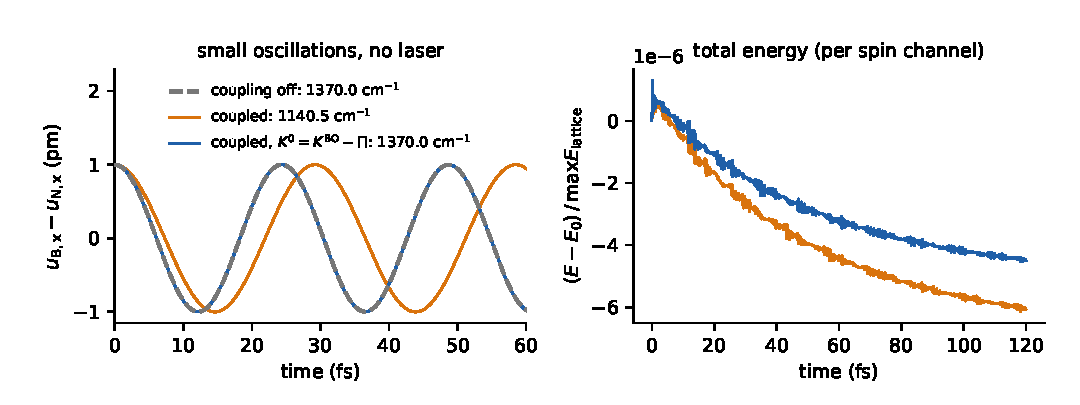
\includegraphics[width=\textwidth]{small_oscillations.pdf}
\caption{Left: free oscillation of the relative displacement. Without coupling (dashed, exactly under the blue curve)
the frequency is that of the dyn file. With coupling the electrons soften the mode. When their static response is
removed from $K$, the dyn frequency is recovered. Right: total energy, per spin channel, relative to the largest
lattice energy. The drift of a few $10^{-6}$ over 120 fs is the error of RK4 at $\Delta t=0.05$ fs.}
\label{fig:small}
\end{figure}

\begin{center}
\small
\begin{tabularx}{\textwidth}{@{}>{\raggedright\arraybackslash}p{5.6cm}L@{}}
\toprule
Test & Result \\
\midrule
Coupling off, initial displacement & fitted frequency 1370.000 cm$^{-1}$ (input 1370), $|E-E_0|<6\times10^{-15}$ Ha \\
Coupling on, no laser, lattice at rest & $|u|\sim10^{-17}$ bohr, $|F|\sim10^{-17}$ Ha/bohr (rounding) \\
Coupling on, initial displacement & 1140.53 cm$^{-1}$. Prediction: the bare frequency computed by the code is 1566.2 and
$\sqrt{1370^2-(1566.2^2-1370^2)}=1140.5$ cm$^{-1}$. Energy conserved to $3\times10^{-6}$ of the lattice energy \\
Same with the static reference & 1369.957 cm$^{-1}$: the static limit is recovered to $3\times10^{-5}$
(non-adiabatic correction, $\omega\ll$ gap) \\
Laser, energy balance & $\max|E-E_0-W| = 1.106\times10^{-6}$ Ha with phonons, $1.107\times10^{-6}$ without
($\max|W|=1.67\times10^{-4}$): the residual is the trapezoidal integration of $W$, and the lattice terms add no error \\
MPI ranks 1, 2, 4 & \file{Lattice.txt} identical to $5\times10^{-12}$ \\
Peierls vs gradient gauge & populations differ by 0.26\%, the same with and without phonons ($k$ discretization) \\
Wrong key inside \texttt{"phonons"} & reported, with the suggestion of the correct name \\
\bottomrule
\end{tabularx}
\end{center}

\begin{figure}[h]
\centering
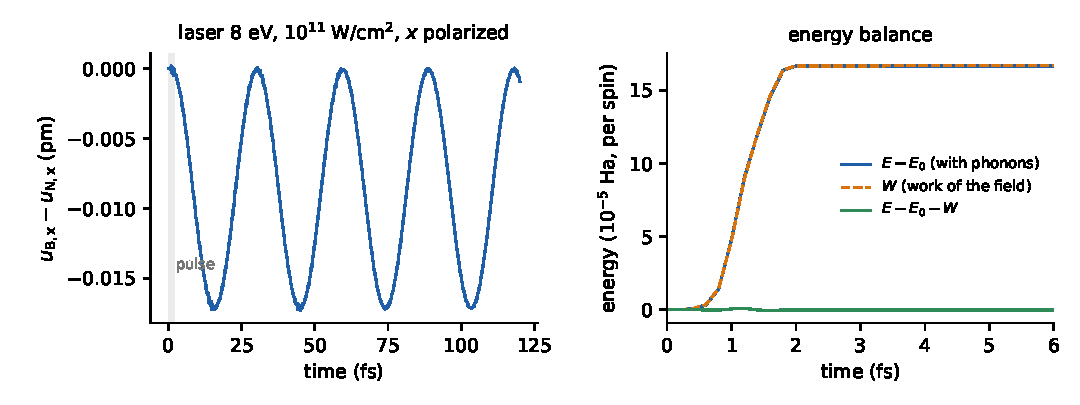
\includegraphics[width=\textwidth]{laser.pdf}
\caption{Laser of 8 eV (above the gap), $10^{11}$ W/cm$^2$, 4 cycles, polarized along $x$, coupling on. Left: the
photoexcited carriers push the $E'$ mode to a shifted equilibrium, around which it oscillates at 1141 cm$^{-1}$ (cosine-like,
displacive excitation). Right: the energy absorbed equals the work of the field, and the residual stays at the level
of the integration error.}
\label{fig:laser}
\end{figure}

\paragraph{Time step.} For the laser run, the maximum relative difference of the displacement from a reference run with
AB4 at $\Delta t=0.005$ fs:
\begin{center}
\small
\begin{tabular}{@{}lcc@{}}
\toprule
Solver & $\Delta t$ (fs) & max relative error of $u$ \\
\midrule
RK4 & 0.05 & $2.4\times10^{-2}$ \\
RK4 & 0.025 & $2.5\times10^{-3}$ \\
RK4 & 0.0125 & $1.7\times10^{-5}$ \\
AB4 & 0.01 & $2.6\times10^{-3}$ \\
\bottomrule
\end{tabular}
\end{center}
RK4 and AB4 converge to the same result. The errors are relative to a reference that has its own error, so the last row
of RK4 should not be read as an order of convergence. With a laser of 8 eV, $\Delta t=0.05$ fs is too coarse for a
percent accuracy (the electronic frequencies set the step, not the phonon). Also, the AB4 run at $\Delta t=0.02$ fs was
correctly stopped by the stability check.

\subsection{Adiabatic reference}
Same model with the HSEX mean field ($\epsilon=1$, $r_0=10$~\AA), without and with the laser:
\begin{center}
\small
\begin{tabularx}{\textwidth}{@{}>{\raggedright\arraybackslash}p{5.6cm}L@{}}
\toprule
Test & Result \\
\midrule
IPA, \texttt{static} & identical to the previous \texttt{subtract} ($10^{-19}$ bohr): without mean field $\Pi=\Pi^{\rm IPA}$ \\
IPA and HSEX, \texttt{dynamic}, no laser & 1370.000 cm$^{-1}$ exactly ($\rho=\rho_{\rm BO}$), energy conserved to $10^{-15}$ Ha \\
HSEX, \texttt{none}, no laser & 1006.4 cm$^{-1}$: strongly softened (bare frequency with the HSEX response: 1655 cm$^{-1}$,
against 1566 with the IPA response, i.e. excitonic enhancement of $\Pi$) \\
HSEX, \texttt{static}, no laser & 1369.67 cm$^{-1}$: the interacting static response gives back the frequency of ph.x \\
HSEX, energy without laser & drift linear in time, reduced 18 times by halving $\Delta t$: it is the RK4 error (fast
electronic coherences excited by the sudden displacement), not the bookkeeping \\
HSEX + laser, three references & energy balance $9.6\times10^{-4}$ in all three (as without phonons, sampling of $W$);
\texttt{static} and \texttt{dynamic} differ by 0.3\% on the displacement; \texttt{none} differs from them by 77\%
(maximum pointwise difference: it oscillates at the softened frequency and goes out of phase) \\
MPI 1, 2, 4 ranks, \texttt{static} and \texttt{dynamic} & displacement and force identical to $3\times10^{-12}$ \\
\bottomrule
\end{tabularx}
\end{center}

\begin{figure}[h]
\centering
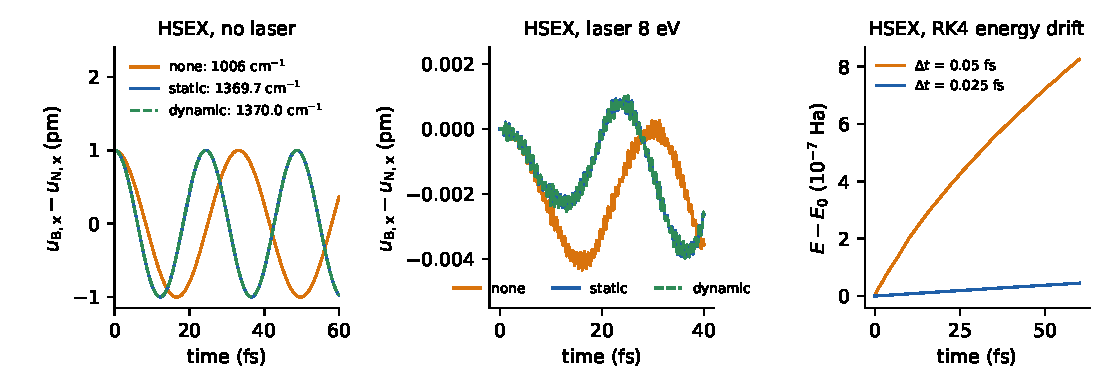
\includegraphics[width=\textwidth]{adiabatic_reference.pdf}
\caption{HSEX. Left: small oscillations without laser: with \texttt{none} the mode is softened to 1006 cm$^{-1}$, with
\texttt{static} and \texttt{dynamic} the frequency of ph.x is recovered. Centre: coherent phonon driven by the laser:
\texttt{static} and \texttt{dynamic} almost coincide. Right: energy drift without laser (\texttt{none}) for two time
steps: fourth-order convergence.}
\label{fig:adiabatic}
\end{figure}

\paragraph{Regressions.} With phonons off all the existing tests pass (hBN IPA/HSEX, Si IPA/HSEX, Magnus, decay,
GaAs, LiF, 1 and 2 ranks), as do the unit tests of the time steppers. The absorbance comparison could not run locally
because \texttt{plotly} is missing, but it is computed from \file{Velocity.txt}, which matches. The three new CI tests pass
(\texttt{hBN\_HSEX\_phonons} also with 4 ranks); \texttt{hBN\_HSEX\_phonons\_static} uses $\Delta t=0.0125$ fs to keep the
RK4 drift of the energy below the tolerance. In the laser HSEX test \file{printresolution} was set to 2: with 4 the balance residual (0.77\%, the same
without phonons) is only due to the sampling of the power, and was too close to the 1\% tolerance.

\section{Unscreening of the coupling of EPW}\label{sec:unscreening}
The right coupling for the Hamiltonian is screened by everything except the electrons of the model (as in constrained
RPA/DFPT). In the static limit the model responds with $\delta\rho=\chi_0V$ to $V=g^{\rm b}+\Sigma[\delta\rho]$; asking
$V=g^{\rm s}$ gives, exactly and without iterations,
\begin{equation}
g^{\rm b}_\mu = g^{\rm s}_\mu - \Sigma\big[\chi_0\,g^{\rm s}_\mu\big],
\end{equation}
computed once at the beginning (\texttt{Lattice::unscreen\_coupling}, with the same $\chi_0$ and $\Sigma$ of the static
response). Then in the static limit the electrons feel the coupling of DFPT, and with the static reference the lattice has
the force constants of ph.x. The recap prints the relative size of the correction and, with the static reference, the
check $\max|g^{\rm b}+\Sigma[\delta\rho]-g^{\rm s}|/\max|g^{\rm s}|$. On the synthetic hBN with HSEX: correction
35\%, check $1.2\times10^{-11}$, frequency of ph.x recovered (CI test \texttt{hBN\_HSEX\_phonons\_screened}).
Stock ph.x refuses \texttt{lnoloc} for phonons (\file{phq\_readin.f90}), so the bare route was never viable as it was
written in the previous version of this note.

\section{Validation on the real hBN (QE \texorpdfstring{$\to$}{->} EPW \texorpdfstring{$\to$}{->} EDUS)}\label{sec:validation_epw}
Same tests as section~\ref{sec:validation}, now with the coupling computed by EPW, which the synthetic model cannot
check: the unscreening (the synthetic data do not distinguish $g^{\rm s}$ from $g^{\rm b}$), the rigid translation in
$g$ ($\sum_\kappa g_\kappa = 0$ by construction in the synthetic model) and the gauge of the Wannier functions of EPW.
The runs are in \file{~/simulations/hBN_EDUS_phonons}; they are written and analysed by \file{epw_validation.py}
(\texttt{run} and \texttt{analyze}, numbers in \file{data_epw.json}, figures by \file{make_figures_epw.py}). The
\file{README.md} of that directory lists every run with what it was meant to show.

\paragraph{Setup.} Monolayer hBN, PBE, $a=4.743$ bohr, 80 Ry, $12\times12$ $k$ points, \texttt{assume\_isolated = '2D'}.
ph.x at $\Gamma$ only ($E'$ at 1349.535 cm$^{-1}$, $A_2''$ at 808.94 cm$^{-1}$). EPW 6.1 with $n_q=1$, two $p_z$ Wannier
functions (spread 1.94 \AA$^2$), whose \file{hbn_tb.dat} is the \texttt{tb\_file} of EDUS (IPA gap 4.67 eV). Initial
displacement 0.01~\AA{} of B along $x$ and N opposite, with the center of mass at rest (the $E'$ mode). HSEX with
$\epsilon=2$, $r_0=10$~\AA. Laser 5.5 eV, $10^{11}$ W/cm$^2$, 4 cycles, along $x$. RK4, $\Delta t = 0.01$ fs.

\begin{center}
\small
\begin{tabularx}{\textwidth}{@{}>{\raggedright\arraybackslash}p{3.3cm}>{\raggedright\arraybackslash}p{5.2cm}L@{}}
\toprule
Run & Effect we want to see & Result \\
\midrule
\multicolumn{3}{@{}l}{\emph{Setup of the coupling (recap of every run)}} \\
gauge & EPW and EDUS use the same Wannier functions & $\max|H_{\rm EPW}-H_{\rm tb}| = 1.1\times10^{-7}$ eV \\
translation in $g$ & the real coupling has $\sum_\kappa g_\kappa\neq0$ (section~\ref{sec:screening}); after the correction no force on the center of mass & $\max|\sum_\kappa g|/\max|g| = 2.0$ before, $\Pi$ satisfies the sum rule to $6\times10^{-17}$ Ha/bohr$^2$ after \\
unscreening & with HSEX $g^{\rm b}$ differs from $g^{\rm s}$; in IPA they coincide & correction 22\% (HSEX), 0 (IPA) \\
\midrule
\multicolumn{3}{@{}l}{\emph{IPA, no laser}} \\
\texttt{ipa\_off} & coupling off: the lattice alone oscillates with $K^{\rm BO}$ of ph.x & 1349.531 cm$^{-1}$ (ph.x 1349.535, fit), energy to $2\times10^{-13}$ \\
\texttt{ipa\_rest} & coupling on, lattice at rest, no laser: no force, because only $\rho-\rho_0$ pushes & $|u|=5\times10^{-16}$ bohr, $|F|=4\times10^{-16}$ Ha/bohr \\
\texttt{ipa\_none} & response counted twice: the mode softens to $\sqrt{2\omega_{\rm BO}^2-\omega_0^2}$ & 873.68 cm$^{-1}$, predicted 873.40 from $\omega_0 = 1696.9$ (bare frequency printed by the code) \\
\texttt{ipa\_static} & static limit gives back ph.x & 1349.588 cm$^{-1}$ ($+4\times10^{-5}$), energy to $3\times10^{-9}$ \\
\texttt{ipa\_static\_u0.5}, \texttt{\_u0.25} & separate the non-adiabatic correction (amplitude independent) from the non-linear response ($\propto u^2$) & fit $\omega=\omega_K+a+b\,s^2$: $a=-0.24$ cm$^{-1}$ (softening, as expected in an insulator), $b=+0.30$ cm$^{-1}$ at 0.01~\AA. The hardening of \texttt{ipa\_static} is the non-linear term \\
\texttt{ipa\_dynamic} & $\rho=\rho_{\rm BO}$ without laser: exactly $K^{\rm BO}$ & 1349.531 cm$^{-1}$, energy to $3\times10^{-13}$ \\
\midrule
\multicolumn{3}{@{}l}{\emph{HSEX ($\epsilon=2$), no laser}} \\
\texttt{hsex\_none} & softening larger than in IPA (excitonic enhancement of $\Pi$) & 989.96 cm$^{-1}$, predicted 990.86 from $\omega_0=1631.1$ \\
\texttt{hsex\_static} & static limit of the interacting model gives back ph.x (tests the unscreening of the real $g$) & 1348.80 cm$^{-1}$; with \texttt{\_u0.5}, \texttt{\_u0.25}: $a=-0.36$, $b=-0.37$ cm$^{-1}$, so the harmonic static limit is ph.x to $3\times10^{-4}$ \\
\texttt{hsex\_dynamic} & exactly $K^{\rm BO}$ & 1349.531 cm$^{-1}$, energy to $4\times10^{-13}$ \\
\texttt{hsex\_*\_dt2} & the energy drift of \texttt{none}/\texttt{static} is the RK4 error & drift $2.0\times10^{-5}\to6.1\times10^{-7}$ (\texttt{none}) and $1.3\times10^{-5}\to4.2\times10^{-7}$ (\texttt{static}) halving $\Delta t$ \\
\midrule
\multicolumn{3}{@{}l}{\emph{Laser}} \\
\texttt{ipa\_laser}, \texttt{\_nophonons} & energy balance $E-E_0=W$ unchanged by the lattice & $\max|E-E_0-W| = 4.30\times10^{-6}$ Ha with and without phonons ($W=4.3\times10^{-4}$) \\
\texttt{ipa\_laser} & coherent $E'$ phonon after the pulse at the frequency of ph.x & 1349.52 cm$^{-1}$; amplitude $5\times10^{-4}$ pm, offset $1.5\times10^{-4}$ pm: not the $1-\cos$ of a displacive mode ($E'$ is not totally symmetric, see below) \\
\texttt{hsex\_laser\_none}, \texttt{\_static}, \texttt{\_dynamic} & balance in all three; \texttt{static} $\approx$ \texttt{dynamic}, \texttt{none} out of phase & balance $2.92\times10^{-6}$ Ha in all three and without phonons; \texttt{static} vs \texttt{dynamic} 0.2\%, \texttt{none} vs \texttt{static} 47\% \\
\texttt{*\_np2}, \texttt{*\_np4} & independent of the MPI ranks & $10^{-12}$ (IPA), $10^{-11}$ (HSEX) \\
\texttt{ipa\_laser\_gradient}, \texttt{\_nophonons\_gradient} & Peierls vs gradient gauge: same difference with and without phonons & populations differ by 0.46\% with, 0.41\% without phonons; effect of the phonons on the populations 0.11\% \\
\texttt{ipa\_laser\_rk\_*}, \texttt{\_ab\_*} & convergence in the time step against AB4 at 0.005 fs & RK4: $9.7\times10^{-2}$ (0.05 fs), $5.6\times10^{-3}$ (0.025), $2.9\times10^{-5}$ (0.0125), $2.4\times10^{-4}$ (0.01); AB4 0.01 fs: $5.9\times10^{-3}$ \\
\bottomrule
\end{tabularx}
\end{center}

\begin{figure}[h]
\centering
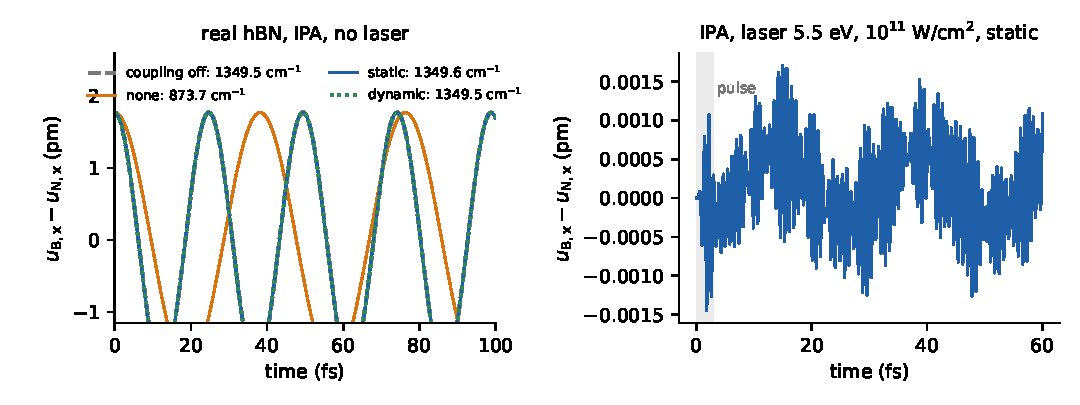
\includegraphics[width=\textwidth]{epw_ipa.pdf}
\caption{Real hBN, IPA. Left: free oscillation of the $E'$ mode for the three adiabatic references and with the
coupling off. Right: coherent $E'$ phonon driven by the laser (static reference).}
\label{fig:epw_ipa}
\end{figure}

\begin{figure}[h]
\centering
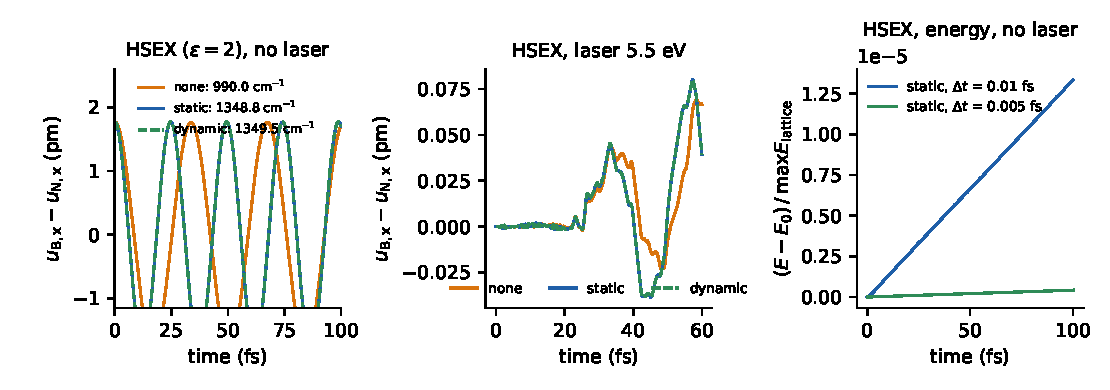
\includegraphics[width=\textwidth]{epw_hsex.pdf}
\caption{Real hBN, HSEX with $\epsilon=2$. Left: free oscillation. Centre: laser. Right: energy without laser for two
time steps.}
\label{fig:epw_hsex}
\end{figure}

\paragraph{The first runs with $\epsilon=1$ (directory \texttt{edus/}).} With HSEX at $\epsilon=1$ the DFT bands of this
model are excitonically unstable (section~5 of \file{EHRENFEST.md}): with the coupling off
(\texttt{hsex\_nocoupling}) and no laser the conduction population grows from rounding to 2\% in 30 fs, the same with
$\Delta t/2$, so it is the model and not the time stepper. With $\epsilon = 1.5$, 2, 3 it stays at $5\times10^{-16}$:
this is why the validation uses $\epsilon=2$. The runs with the coupling at $\epsilon=1$ (\texttt{hsex\_static},
\texttt{hsex\_bare\_static}) reach 70\% of population and are not meaningful; \texttt{hsex\_bare\_static} shows also that
using the screened files as $g^{\rm b}$ (\texttt{coupling = "bare"}) gives a bare frequency of 1868.7 cm$^{-1}$ against
1544.4 with the unscreening, i.e.\ the screening of the model counted twice.

\paragraph{What these tests do not show.} The $E'$ mode of hBN is not totally symmetric: a population of carriers with
the symmetry of the crystal exerts no force on it, and the laser pushes it only through the anisotropy of the
excitation along $x$. The result is a small oscillation without the shifted equilibrium of the displacive mechanism, and
$E'$ is also infrared active, whose direct driving by $Z^*$ is not implemented. A clean test of the displacive
excitation of coherent phonons (DECP: $u(t)\propto1-\cos\omega t$, amplitude linear in the absorbed energy) needs a
totally symmetric mode, e.g.\ $A_1'$ of monolayer MoS$_2$.

\section{What is missing and open points}
\begin{itemize}
\item \textbf{Static limit on the real hBN} (solved, section~\ref{sec:validation_epw}): the hardening of $4\times10^{-5}$
  of \texttt{static} is the non-linear response at 0.01~\AA; the harmonic part is a softening of 0.24 cm$^{-1}$, as
  expected.
\item \textbf{DECP on a totally symmetric mode} (MoS$_2$ $A_1'$), the first physical effect to compare with experiment.
\item The static response uses linear mixing: for strongly bound excitons (spectral radius of $\chi_0\Sigma$ close to 1)
  it may need a better solver (Anderson mixing or GMRES).
\item $q\neq\Gamma$ (needs $\rho(k,q)$, EHRENFEST.md section 7), Born effective charges for the direct infrared driving
  of polar modes, GPU, Magnus with the lattice, dynamical matrix in xml format.
\end{itemize}

\paragraph{Practical notes.} The directory \file{build/} still points to the old path \file{EDUS_2.0}: it needs a new
\texttt{cmake}. \file{ci-test/outputs/} is in \file{.gitignore}, so the new references must be added with
\texttt{git add -f}. None of this is committed yet.

\end{document}
